% 第 3 章 系统测试与结果
% 本章引用键（实际使用）：fips203, kyberslash, clangover, dudect, rtlf, microwalk, binsec
% 表号接第 2 章（表 3–5），本章从表 6 起；图号接第 2 章（图 1–3），本章为图 4、5、7–10
% 图 6 按定稿删除，90 格数据保留为表 8
\setcounter{table}{5}
\setcounter{figure}{3}

\section{系统测试与结果}

\subsection{测试方案与环境}
% A-30 计时精度与环境
% A-31 运行批次
% A-26 优化级别
% A-01 M1 主结果
% B-08 运行批次合计

测试分六组，每组回答题面条目中的一个问题；环境是一台 x86\_64 裸金属，所有时间结论只在这台机器上成立。六组是功能与语义等价、检测与定位、防护复测、功效与稳健性、性能、跨环境与多工具。分组按“回答哪一个问题”划分，不按工具划分：同一份原始数据可以在不同组里被引用，结论只在其所属组内成立。

六组与题面的对应关系：功能与语义等价对应第 1 条，检测与定位对应第 3--5 条，防护复测对应第 6、7 条，功效与稳健性对应第 4、8 条，性能对应第 8 条，跨环境与多工具对应第 9、11 条；第 2、10 条贯穿所有组。

表~\ref{tab:env} 给出七项环境要素。处理器、操作系统、编译器、动态分析、形式化、计时源与频率控制各自固定；换掉其中任何一项，时间结论都要重测。% A-30

\begin{table}[H]
\centering
\caption{测试环境}
\label{tab:env}
{\small
\begin{tabularx}{\textwidth}{|>{\raggedright\arraybackslash}p{2.3cm}|>{\raggedright\arraybackslash}X|}
\hline
项目 & 配置 \\
\hline
处理器 & AMD Ryzen 9 9950X（x86\_64），SMT 开启，未配置 isolcpus \\
\hline
操作系统 & Ubuntu 24.04.4 LTS，Linux 6.17，amd\_pstate 频率驱动 \\
\hline
编译器 & clang 18.1.3（主构建）；gcc 13.3.0 已安装但未用于对照实验 \\
\hline
动态分析 & Valgrind 3.22.0（Memcheck）；Valgrind 3.25.1 + KyberSlash varlat 补丁；Intel Pin 3.28（Microwalk） \\
\hline
形式化 & Binsec 0.11.3 + Z3 4.15.3 \\
\hline
计时源 & 单调时钟（完整解封装）；原始单调时钟（M4 比较调用） \\
\hline
频率控制 & 关闭睿频，性能策略，频率上下限均为 4,300,000 kHz，绑核 CPU2 / CPU6 \\
\hline
\end{tabularx}
\par\smallskip
{\footnotesize \textbf{表注：}单台 x86\_64 裸金属、clang 18.1.3、锁频 4.30 GHz。gcc 只安装未参与对照，结论不覆盖 gcc；SMT 开启且未配置 isolcpus，后台约 39 个服务在运行，单次调用的量化尺度约 10 ns。}
}
\end{table}

表~\ref{tab:env} 证明每组实验都有固定的处理器、编译器、工具版本与频率工作点；它不证明这些条件覆盖其他机器。

操作系统与频率驱动最容易被忽略：锁频协议通过 sysfs 写频率上下限，换内核或换驱动，20 次探针的读数就可能落在不同工作点。编译器版本同样是背景信息：M1 的分支是 clang 18 在特定选项下的产物，换编译器等于换被测对象。环境表的作用是让“未检出”有明确的工具边界。

图~\ref{fig:matrix} 把五个模块、三类对象与七类实验环境排在同一张矩阵上。矩阵的行是实验类别，列是模块；空格不是遗漏，是该模块在该类实验中没有对象或不适用。% A-26--A-31

\begin{figure}[htbp]
\centering
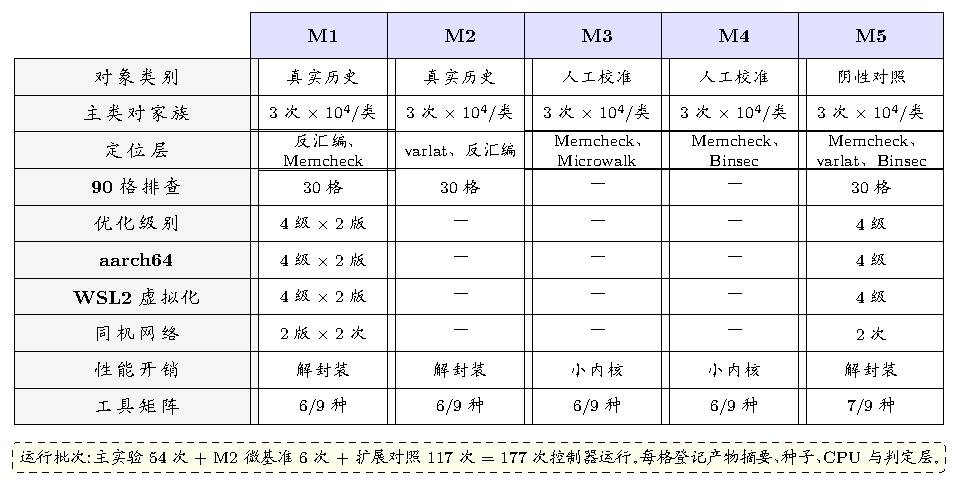
\includegraphics[width=0.98\textwidth]{assets/fig4.pdf}
\caption{实验矩阵与运行批次}
\label{fig:matrix}
\par\smallskip
{\footnotesize 图注：五个模块、三类对象、锁频/不锁频、优化级别、架构与网络各自独立登记。矩阵的空格表示该模块在该类实验中没有对象，不表示未执行；未执行项在正文单列。}
\end{figure}

矩阵的每一格都绑定产物摘要、种子、CPU 与判定层。图~\ref{fig:matrix} 证明每一项结论都有对应的对象、环境与判定层；它不证明这些组合覆盖了所有环境，矩阵之外的组合没有数据。

正式采集分三批：平台家族 54 次控制器运行、M2 微基准 6 次、收尾 117 次（格式破损 18、性能 54、优化级别 36、锁频对照 9），合计 177 次。一次控制器运行是一次经过计划校验、频率放行与退出恢复的采集单元；M1 的封存数据不计入这 177 次，统计口径仍按当时冻结的家族。% A-31 % B-08

被拒绝的运行与未执行项分开登记。优化级别实验中有 1 次运行因 20 次探针的频率跨度 54,629 kHz 超过 50,000 kHz 阈值被控制器拒绝，换名重跑后计入；性能批次有 1 次运行跨度 50,310 kHz 略超阈值，20 个采样值仍在 ±2\% 带内，已如实登记。未执行项包括 GCC 对照、-O1/-Oz/-Og 三个优化级别、第三架构、isolcpus 与关闭 SMT、真实远程网络、第二台测量机、Microwalk 扩展到 M1/M2、Binsec 覆盖完整解封装、面向 CI 的回归门禁。这些项目只写“未执行”，不并进阴性。% A-26 % A-31

M1 的数据是同一台机器、同一套锁频规程下的前期封存结果，不是与 M2--M5 同一批采集；引用时单独标注。第二台真实测量机没有部署，所有时间结论只来自这一台 x86\_64 裸金属；aarch64 只构成第二架构，不是第二台测量机（3.11）。这两条决定适用范围。% A-01

\subsection{功能与语义等价测试}
% A-33 M1 功能向量
% A-34 M2/M3/M5 功能向量
% A-35 修复等价与额外输入

功能测试先证明“被测对象仍是 ML-KEM”，再谈侧信道；修复版本必须与未修版本逐字节等价。被测对象的口径并不相同：M1 是 FIPS 203 初始公开草案的可移植 C 路径，M2 是历史 Kyber768 参考实现，M5 对应最终标准。三者的功能向量不能混用同一套期望值；M1 的密钥生成差异就是口径差异的直接结果。\cite{fips203}

表~\ref{tab:function} 把五组功能结果列在一起。% A-33--A-35

\begin{table}[H]
\centering
\caption{功能正确性与语义等价}
\label{tab:function}
{\small
\begin{tabularx}{\textwidth}{|>{\raggedright\arraybackslash}p{2.5cm}|>{\raggedright\arraybackslash}p{3.5cm}|>{\raggedright\arraybackslash}X|}
\hline
对象 & 测试向量 & 结果与说明 \\
\hline
M1 两版 & NIST ACVP 转换的 ML-KEM-768 向量 & 执行 60 例通过 35：encaps 25/25、decaps 10/10（含 5 例隐式拒绝）通过；keygen 0/25 未通过，原因是 liboqs 0.10.0 实现 FIPS 203 初始公开草案，其 K-PKE.KeyGen 的哈希输入不含最终稿新增的参数集域分隔字节；另有 20 例密钥校验因封装层无对应入口记为不适用 \\
\hline
M2 两版 & Kyber round3 官方 KAT & 100/100；普通构建与 ASan/UBSan 构建测试各 7/7 \\
\hline
M3、M5 & NIST 独立向量 & 各 80/80（含隐式拒绝用例） \\
\hline
修复等价性 & 同一驱动、同一公开输入 & 三对“未修 / 已修”实现的逐例输出摘要 diff 全空 \\
\hline
额外输入 & 一半随机密文、一半逐字节篡改 & 隐式拒绝 1000/1000 按 FIPS 203 或 round3 规范生效 \\
\hline
\end{tabularx}
\par\smallskip
{\footnotesize \textbf{表注：}修复前后功能等价；M1 keygen 0/25 来自 ipd 与最终稿的域分隔差异，不是实现错误。}
}
\end{table}

keygen 0/25 需要单独解释。liboqs 0.10.0 实现的是 FIPS 203 初始公开草案，草案的 K-PKE.KeyGen 在哈希输入中没有最终稿新增的参数集域分隔字节；用最终稿生成的向量去核对，密钥生成必然对不上。这是标准版本差异，不是实现错误。0/25 是标准版本差异，35/60 是可核对的通过数；两种简化都会改变对象口径。

这 60 例的构成需要写清楚。encaps 25/25 覆盖封装路径的接受分支；decaps 10/10 里含 5 例隐式拒绝，覆盖比较失败后返回假密钥的路径；keygen 0/25 全部落在密钥生成；另有 20 例密钥校验因为该封装层没有对应入口，只能记为不适用。35 通过、25 未通过，合计 60；另有 20 例不适用，单列，不与这 60 例混算。这个口径与台账的四种状态一致：不适用不是失败，也不是通过。

20 例密钥校验记为不适用，是因为该封装层没有对应入口，不是测试没做。不适用与未通过的区别在报告里必须写清楚：前者是“这个接口不提供这项检查”，后者是“提供了但结果不对”。把 20 例不适用并进 35/60 的通过率，会把分母弄错；把 0/25 的 keygen 并进“实现错误”，会把标准版本差异写成缺陷。

M2 用 Kyber round3 官方 KAT，100/100；普通构建与 ASan/UBSan 构建各 7/7。M3 与 M5 用 NIST 独立向量，各 80/80，含隐式拒绝用例。三套对象的向量来源不同，是因为它们的标准版本不同：M2 是历史 Kyber768，只能用 round3 的 KAT；M5 对应最终标准，用 NIST 向量；M3 基于 M5 基线，向量与 M5 同源。把三套向量混在一起统计“总通过率”没有意义，表~\ref{tab:function} 因此按对象分行。

三对未修/已修实现的逐例输出摘要 diff 全空，说明修复没有改动算法语义。修复涉及三类改动：把分支改成掩码选择、把除法改成乘法与移位、把人工夹具的查表或提前返回改成固定路径；改动只落在执行路径上，不落在输出上。逐例摘要 diff 比“再跑一遍 KAT”更强：KAT 只比较最终共享密钥，摘要 diff 还把中间输出与返回码一起比较；任何一处字节变化都会留下痕迹。

1000 例额外输入（一半随机密文、一半逐字节篡改）中，隐式拒绝 1000/1000 按 FIPS 203 或 round3 规范生效；这条测试覆盖的是失败路径，不是接受路径。随机密文检验一般路径上的解析与拒绝，逐字节篡改检验比较逻辑在单个字节不同时的行为；两类输入都不接触私钥内容，只检验失败路径是否按规范返回假密钥。1000/1000 说明失败路径没有被修复破坏，不说明失败路径的耗时与成功路径不可区分；后者属于 3.3 的计时层。

ASan/UBSan 构建的 7/7 是另一条证据。普通构建只证明功能正确，消毒器构建还要证明没有越界、未定义行为与内存错误；7/7 说明修复没有引入这类问题。消毒器构建的性能不适合计时，功能测试只在普通构建上做计时，两者分开登记。

表~\ref{tab:function} 证明三对修复没有改动算法语义，M1 的 0/25 是标准草案版本差异；它不证明任何实现是常数时间，也不证明这些向量覆盖了全部输入。功能等价是侧信道结论的前提：如果修复改变了输出，“修复后不可区分”就可能只是算法变了，而不是泄漏消失了。功能测试的另一条边界是向量集：NIST ACVP 与 round3 KAT 覆盖规范路径，不覆盖所有畸形输入；畸形输入由 3.8 的两组对照单独处理。向量集的来源与版本见附录 B，功能结论只覆盖这些向量集。

\subsection{端到端可区分性}
% A-01--A-08 五模块主结果
% A-09--A-14 统计判定与 dudect
% A-16 RTLF
% B-01 效应占比
% B-04 RTLF 数据集
% B-07 主类对样本

预注册 Holm 家族中，只有 M1 未修主类对与 M4 vulnerable 臂被拒绝；M2、M3、M5 的家族均未拒绝任何检验。图~\ref{fig:forest} 把七个类对的均值差与 95\% 区间放在同一把尺子上：M1 未修与 M4 vulnerable 的区间不含 0，其余五个区间含 0。% A-01--A-08

\begin{figure}[htbp]
\centering
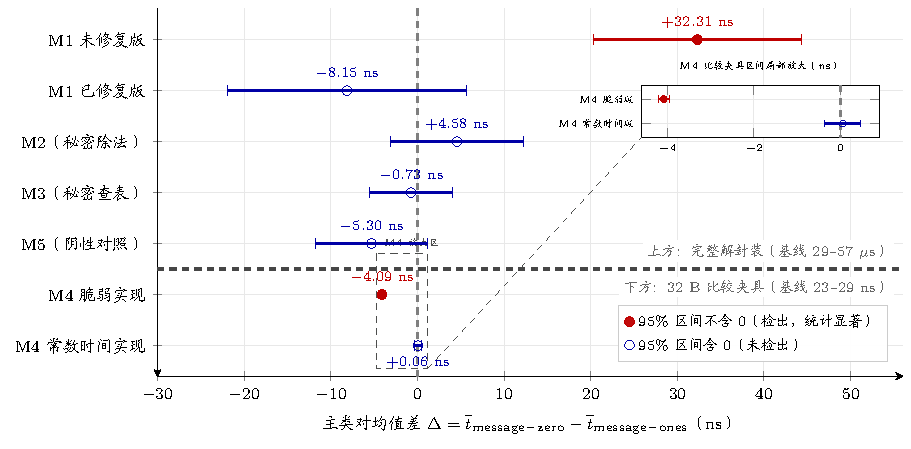
\includegraphics[width=0.98\textwidth]{assets/fig5.pdf}
\caption{五模块主类对均值差与 95\% 区间}
\label{fig:forest}
\par\smallskip
{\footnotesize 图注：M1 与 M4 vulnerable 臂区间不含 0，其余模块未检出。区间为三次独立运行的逆方差合并结果；M4 是 32 B 比较调用，数值不可与完整解封装直接比较。}
\end{figure}

家族的构成决定了门槛。M1、M2、M3、M4 各 6 项，M5 3 项；每个模块的 6 项来自 3 次独立运行 $\times$ 2 个版本或臂。Holm 是逐步下降校正：家族内 $p$ 值升序排列，第 $i$ 个与 $\alpha/(m-i+1)$ 比较，一旦某一步不拒绝就停止。M1 的 $m=6$，最小 $p$ 的门槛是 $0.05/6\approx0.00833$；M4 的 $m=6$，门槛相同；M5 的 $m=3$，门槛是 $0.0167$。门槛在采集前写进计划，不随观测到的 $p$ 值变化。

先看 M1。三次独立运行的均值差为 +39.337、+31.117、+22.337 ns，三个 95\% 区间都不含 0；逆方差合并为 +32.311 ns，区间 [20.282, 44.339]。Holm 家族 $m=6$，最小 $p=1.30\times10^{-5}$，低于阈值 0.00833，是家族中唯一被拒绝的检验。效应占完整解封装均值 57,010.7 ns 的 0.0567\%，约 0.06\%；32 ns 在 10 ns 的最小步进下只有 2--3 个分辨率单位，单次调用不可分辨，结论靠每类 10,000 次、三次运行。dudect 的最大 $t$ 为 26.41、40.64、14.92，RTLF 在未修臂报告差异、在已修臂未报告差异，方向与 Welch 检验一致。% A-01 % A-09 % A-11 % B-01 % B-07

三次运行的方向一致，比单次拒绝更重要。三次分别换种子、换物理核：同核不同种子两次，同种子不同核一次；三次都给出正号、区间都不含 0，说明结论不依赖某一组输入或某一个核的局部状态。反过来说，如果三次方向不一致，即使合并后拒绝零假设，也要按预注册规则登记为不稳定，不能挑一次最有利的运行写进结论。M1 的三次结果没有触发这条规则。

效应大小与统计判定要分开读。32.311 ns 只占 57,010.7 ns 的 0.06\%，在绝对值上很小；它的统计判定来自每类 10,000 次、三次运行与预注册家族，不来自效应大。把“拒绝零假设”当成“效应大”会误导读者：这个效应在单次调用上不可分辨，在本地锁频、大样本下才可分辨；远程或小样本下可能完全看不到。

M4 的阳性更强。vulnerable 臂三次运行的原始 $p$ 为 0、$9.23\times10^{-25}$、$3.14\times10^{-22}$；0 是双精度下溢，正文写“小于最小可表示值”。Holm 家族 $m=6$，拒绝 3 项，全部来自 vulnerable 臂；合并差 $-4.089$ ns，区间 [$-4.215$, $-3.963$]。ct 臂合并差 +0.055 ns，区间 [$-0.363$, 0.473]，原始 $p$ 为 0.386、0.438、0.399，三项都不拒绝。dudect 的最大 $t$ 从 vulnerable 臂的 356.6、396.9、395.6 降到 ct 臂的 2.06、1.90、2.27。M4 是 32 B 比较调用，用原始单调时钟计时，数值不可与完整解封装的 32 ns 直接比较。% A-06 % A-07 % A-10 % A-12

M4 的区间窄得几乎看不见，是因为比较调用的方差远小于完整解封装。32 B 比较的基线远小于完整解封装，单次调用没有 NTT、采样与序列化的开销，噪声源少，标准误小；同样的每类 10,000 次，M4 的 MDE 只有 0.19--1.19 ns，而完整解封装的 MDE 在几十纳秒。区间窄不等于效应大：$-4.089$ ns 在绝对值上只有 M1 的八分之一，但它的信噪比高，所以在图上反而更醒目。

效应绝对值与可检出性强弱并不同向：M4 只有 4 ns，MDE 低到 1.47 ns，信噪比高；M1 的 32 ns 更大，完整解封装的方差也大，MDE 高到 31.39 ns，信噪比反而低。判断可区分性要看区间与 MDE，不看点的位置。

M2 的家族没有拒绝项。完整解封装合并差 +4.58 ns，区间 [$-3.08$, 12.25]，含 0；按臂描述，未修臂 +12.35 ns、已修臂 $-11.20$ ns，$I^2=58.3\%$。两个方向相反、异质性偏高，读作臂间漂移，不读作除法泄漏。按臂合并值不属于预注册的 6 个家族成员；家族成员是三次运行的逐次检验，按臂值只作描述。

主类对不是为除法操作数设计的：message-zero 与 message-ones 只让解密消息的位不同，除法的被除数是否随消息位系统变化没有控制；这一条在 3.7 的检测预算里再展开。M2 的 dudect 阳性落在已修臂（4.68、3.05、3.66 对 36.27、30.94、61.91），不能归因于除法；3.12 把它作为单工具误读的例子。% A-03 % A-04 % A-13

M2 的按臂描述还暴露了主类对的设计问题。未修臂 +12.35 ns、已修臂 $-11.20$ ns，两个方向相反；如果主类对真的触发了除法，两个臂应该同向，只是幅度不同。方向相反说明两臂的差异更多来自运行间的漂移，而不是同一个机制。$I^2=58.3\%$ 是这种漂移的量化：合并估计只作描述，判定仍以预注册的 Holm 结果为准。

M3 的合并差为 $-0.73$ ns，区间 [$-5.56$, 4.10]，Holm 拒绝 0；M5 的合并差为 $-5.30$ ns，区间 [$-11.77$, 1.16]，家族 $m=3$，拒绝 0。M5 是阴性对照，未检出只说明在本机、本编译产物、本类对与每类 10,000 次的预算下没有看到可区分差异；它不是安全性结论。M3 是人工夹具，on/off 两臂只差人工查表，计时层未检出说明该机制在本机没有被端到端计时分辨出来，不说明查表没有风险。M5 的 dudect 最大 $t$ 为 2.10、1.98、2.82，也在阈值 10 以下，与 Welch 检验同向。% A-05 % A-08 % A-14

M5 的 3 项家族成员没有一项接近门槛：合并差 $-5.30$ ns，区间跨 0，dudect 最大 $t$ 只有 2.10、1.98、2.82，远低于阈值 10。三个来源都指向“本预算下未检出”，但没有一个能证明“没有机制”。阴性对照的价值在于检查工具会不会冤枉好人，不在于证明好人一定没问题。

端到端 $\Delta$ 的符号不能按分支代价模型解释。符号受二进制布局、对齐与指令调度影响；主实验的 +32.3 ns 与优化级别实验的 $-26.16$ ns 采用不同的 $\Delta$ 定义方向，同一机制在不同构建中给出相反符号。本作品只按“区间是否含 0”判定可区分性，不解释符号，也不把符号当作机制证据。% A-01 % A-26

图~\ref{fig:forest} 的纵轴按模块排列，不按 p 值排列。按 p 值排列会让读者以为“上面的模块更重要”；按模块排列，读者可以先看同一模块的未修/已修或不同臂，再看跨模块的比较。M4 的两行挨在一起，就是为了让 vulnerable 与 ct 的区间直接对照。

族外检验给出另一层信息。RTLF 在 $\alpha=0.01$、固定种子与 10,000 次 bootstrap 的设置下，对 M2--M5 的 42 个数据集给出 30 个未检出、12 个检出；检出的 12 个集中在 M2 主类对与 M4 vulnerable 臂及其对照，M3 的 12 个与 M5 的 6 个数据集全部未检出。RTLF 与 Welch 检验比较的对象不同：前者比较分布与分位，后者比较均值；两者不互相替代，也不并入同一个 Holm 家族。\cite{rtlf} % A-16 % B-04

族外检验不并入 Holm，是因为零假设与错误控制方式不同。RTLF 用 bootstrap 控制第一类错误，dudect 用最大 $t$ 的经验阈值，Mona 用箱体分离；把三者塞进同一个 Holm 家族，会得到一个既不是 0.05 也不是 0.01 的混合错误率。它们的位置是交叉印证：同向时增加信心，反向时提示输入类或环境有问题，而不是投票。

dudect 也属于族外。它用在线 $t$ 检验，阈值是上游默认的 10，不转换成 $p$ 值参与 Holm；M1 未修在三批内停止并报告泄漏，已修跑满批次仍为“可能常数时间”；M4 vulnerable 三次都报告泄漏，ct 臂三次都未报告；M5 三次都未报告。\cite{dudect}

主类对是同一份确定性密文的 10,000 次重复，单次运行的区间反映测量噪声，不是密文间的变异；跨种子复测部分弥补这一点，但不等价于在每类内部使用大量不同密文。10 ns 的量化尺度下，32 ns 的效应只有 2--3 个分辨率单位；这不是把 32 ns 说小，而是说明为什么必须用大样本与预注册家族。图~\ref{fig:forest} 不能回答“效应从哪来”。区间只说明两类密文的均值差在本预算下是否可区分，不说明差异来自哪条指令；M1 的差异要结合 3.4 的分支定位才能归因，M4 的差异要结合 3.6 的 ct 臂对照才能确认。把图上的点直接读成“某条指令的代价”，会把统计证据与机制证据混在一起。

图~\ref{fig:forest} 证明在本机、本预算下哪些类对可区分；它不证明机制存在或不存在，不证明可远程利用，也不把 M5 的未检出写成安全。

\subsection{函数级泄漏定位}
% A-17 M1 定位
% A-18 M2 定位
% A-19 M3 定位
% A-20 M4 定位
% A-21 M5 定位
% A-23 残留分支

定位层把每个阳性落到函数、指令或源码行；定位阳性与计时阳性是两件事，必须分开登记。同一个模块可以在定位层阳性、在计时层未检出，M2 就是这种组合；反过来，计时层阳性也必须能回到一条具体指令，否则无法判断修复是否生效。

动态检查的工作方式决定了它能回答什么。秘密标记把私钥中参与解密的 1152 B 与隐式拒绝秘密的 32 B 标成“未初始化”，公开输入保持已初始化；程序在标记下跑完整解封装，工具报告“以秘密值为分支条件”与“以秘密值为访存下标”两类事件。错误数是动态命中次数，上下文数是去重后的源码位置数；同一个循环执行 1280 次会报 1280 个错误，但只算 1 个上下文。报告里同时给两个数，是为了让读者看到“问题分布”而不是“执行次数”。

M1 未修版本的消息编码函数里，编译器把源码中的掩码选择还原成按位测试后条件跳转：先测试消息位，再由条件跳转决定是否写入系数。私钥标记下，Memcheck 报告 1 个秘密条件跳转。修复版本改成置位加条件传送：同一个按位测试之后用置位指令物化消息位，再调用 16 位条件传送辅助函数完成选择；反汇编里条件跳转消失，Memcheck 报告 0。两版的功能输出逐字节相同，说明消失的是执行路径，不是语义。\cite{clangover} % A-17

反汇编上的差别可以逐条读。未修版本是“按位测试 + 条件跳转”：测试结果决定是否跳过写系数；修复版本是“按位测试 + 置位 + 调用条件传送辅助函数”：测试结果被物化成 0 或 1，辅助函数用取负、异或、与、再异或完成选择，不产生依赖秘密的跳转。两条路径的指令数不同，但都不依赖秘密；修复的代价是多了几条算术指令与一次调用，收益是分支消失。

M2 的三处整数除法分别落在消息解码、多项式压缩与向量压缩。未修版本在可变时延检查下报告 1280 errors / 3 contexts；修复版本用乘法与移位替代除法，除法计数从 3 降到 0，可变时延报告 0/0。关闭可变时延检查时，两版都报告 0，说明普通 Memcheck 看不到除法：它只检查秘密是否进入分支或访存下标，不检查指令时延是否随操作数变化。1280 次错误来自同一源码位置的多次执行，3 个上下文才是问题分布。\cite{kyberslash} % A-18

三处除法各自对应一个上下文：消息解码一处、多项式压缩一处、向量压缩一处。三处的被除数都来自解密消息或重加密中间值，除数都是公开模数；修复用乘法与移位替代除法，三处的除法计数同时降到 0。varlat 的 1280 次错误分布在三个上下文上，说明三处都被执行到；如果只修一处，另外两处仍会报错。

可变时延检查的边界也要写清楚。它标记的是“秘密操作数进入可变时延指令”，不是“这条指令一定产生可测差异”。除法在 x86\_64 上的时延是否随操作数变化，取决于处理器微架构、操作数大小与流水线状态；工具能指出“这里有秘密操作数”，不能指出“这里一定泄漏多少纳秒”。M2 的定位阳性与计时未检出并不矛盾：前者是机制层，后者是端到端层，两层的判据不同。

M3 的 Memcheck 报告 1280 errors / 2 contexts，全部落在人工插入的秘密下标读取；off 臂去掉查表后为 0/0。Microwalk 在同一对象上给出互信息 1.922 bits，是全场最高；off 臂为 0.722 bits。Microwalk 只有 5 个公开 testcase、没有重复、没有统计检验，互信息只作定位层的独立佐证，不升级为泄漏量。\cite{microwalk} % A-19

互信息 1.922 bits 的含义是“看过这条指令的访存地址后，对秘密的不确定性平均减少 1.922 bit”。它是关联强度，不是泄漏量；1.922 bits 不能换算成“恢复多少位密钥”。Microwalk 的 5 个 testcase 只覆盖 5 组公开输入，没有重复、没有统计检验；互信息高只说明这条指令与秘密关联强，不说明攻击者能利用它。

M4 的 Memcheck 报告 32 errors / 1 context，落在提前返回的比较行。Binsec 在同一对内核上判 vulnerable 为 insecure，反例地址对应提前返回行；ct 臂判 bounded secure，路径探索完整。把搜索深度限为 5 时，工具返回 unknown，而进程退出码仍是 0；只看退出码会把 unknown 读成安全。M4 只开了控制流与访存检查，未开乘除法检查；它的结论只覆盖这对 32 B 比较内核。\cite{binsec} % A-20

Binsec 的反例地址对应提前返回行，说明工具找到了一条“从第几个字节开始不同”的秘密相关路径。ct 臂的 bounded secure 不是“所有输入都安全”，而是“在入口、终点与公开长度 1--16 B 的范围内，没有找到秘密相关路径”；范围外的输入不在证明里。深度限 5 的 unknown 是另一个边界：工具没有证明不安全，也没有证明安全，退出码却是 0。

M5 在三种动态模式下各做 10 次完整解封装：普通 Memcheck、关闭可变时延、开启可变时延，三者都是 0 errors / 0 contexts。重加密路径的 Binsec 检查中，比较步骤 1088/1088 条路径完成，消息编码 1/1 条路径完成，没有秘密相关控制流；同一配置下 M4 的脆弱内核报告 insecure，说明工具在这套配置里不会把已知脆弱代码判成安全。Binsec 只覆盖重加密比较与消息编码，不覆盖完整解封装的所有性质。% A-21

三种动态模式的分工不同：普通 Memcheck 看分支与访存下标，关闭 varlat 看同一组输入下是否有普通标记错误，开启 varlat 看除法等可变时延指令。三者都是 0/0，说明在这组输入上没有这三类问题；换一组输入，未执行的路径不会被报告。Binsec 的 1088/1088 与 1/1 是路径计数，不是“所有路径都安全”的证明；它只覆盖重加密比较与消息编码两个内核。

定位层的输出要归一化成同一种证据记录：工具与版本、输入集合、命中位置、上下文数、处置结论。同一位置被两类工具命中记两条证据，只有一类命中时保留但不升级为“确认”；归因要求同一位置至少在三次运行中的两次出现，且换种子后仍出现，只出现一次的命中记为“待复核”。

五类工具的回答范围可以排成一条链：反汇编回答“机器码里有没有目标指令形态”，不回答运行时是否真的触发；秘密标记回答“秘密是否进入分支或访存下标”，不回答可变时延指令；可变时延检查回答“秘密是否进入除法等指令”，不回答缓存与分支；轨迹互信息回答“哪些指令与秘密的关联最强”，不回答时序可利用性；有界符号执行回答“给定范围内是否存在秘密相关路径”，不回答范围外的行为。链条上的每一环都只回答一个问题，合起来才覆盖机制层的几个侧面。

这组结果证明机制在该产物、该输入、该工具下存在或不存在；它不证明完整解封装一定可测，也不证明未命中的输入没有机制。M4 是 32 B 比较夹具，不外推到完整解封装；Binsec 是有界验证，只覆盖给定内核与公开长度范围；动态工具只覆盖执行过的输入，0 条报告不是安全性结论。定位阳性与计时阳性分开登记：M1 两层都阳性，M2 定位阳性、计时未检出，M3 定位阳性、计时未检出，M4 两层都阳性，M5 两层都未检出。

\subsection{泄漏源全流程排查}
% A-22 90 格汇总
% A-23 残留分支
% B-06 90 格分解

90 格排查把“六类来源 $\times$ 五个步骤 $\times$ 三个实现”逐格判定。5 个“存在”之外，还有一处更需要解释：官方修复后仍残留的同源分支。判定只有四种：存在、不存在、不适用、未检查。判“存在”必须给出可指认的函数、指令或源码位置以及触发它的输入；判“不存在”必须写明用了哪种检查、覆盖了哪些输入；判“不适用”要求该机制在这一步骤上不可能出现；判“未检查”单列，不并入阴性。

五个步骤是解密、哈希派生、重加密、比较与隐式拒绝。把哈希派生从重加密里拆出来，是因为哈希路径上的问题如果被记到重加密名下，定位只能停在“重加密有问题”这一层；拆开后，每一步都有自己的函数与指令，修复后可以逐格复查。六类来源是敏感分支、提前返回、可变时延指令、秘密下标、数据相关循环与异常路径；三个实现是 M1、M2 与 M5，人工夹具 M3、M4 不进入这张表，因为它们只覆盖单一机制，放进 90 格会把夹具结论与真实实现混在一起。

\setcounter{algorithm}{7}
\begin{algorithm}[H]
\caption{90 格泄漏源排查}
\label{alg:sweep}
\begin{algorithmic}[1]
\Require 实现集合 $\{$M1, M2, M5$\}$；步骤集合 $\{$解密, 哈希派生, 重加密, 比较, 隐式拒绝$\}$；六类来源
\Ensure 90 格判定与证据
\For{每个实现、每个步骤、每类来源}
  \State 检查源码与反汇编
  \State 运行 Memcheck、varlat、Microwalk、Binsec（适用时）
  \State 判定：存在 / 不存在 / 不适用 / 未检查
  \State 记录函数、源码行或指令地址、证据编号
\EndFor
\State 汇总：存在 5 / 不存在 75 / 不适用 10 / 未检查 0
\end{algorithmic}
\end{algorithm}

算法~\ref{alg:sweep} 回答的是每一格在给定产物与检查手段下是否存在机制；它不回答该机制是否能被端到端计时分辨。表~\ref{tab:sweep} 给出汇总。% A-22 % B-06

\begin{table}[H]
\centering
\caption{全流程排查汇总}
\label{tab:sweep}
{\small
\begin{tabularx}{\textwidth}{|>{\raggedright\arraybackslash}p{4.4cm}|*{5}{>{\centering\arraybackslash}X|}}
\hline
实现 & 存在 & 不存在 & 不适用 & 未检查 & 小计 \\
\hline
M1 liboqs 0.10.0（未修 / 982c762） & 1 & 26 & 3 & 0 & 30 \\
\hline
M2 Kyber768（a621b8d / 272125f） & 3 & 24 & 3 & 0 & 30 \\
\hline
M5 mlkem-native b3ba7b3 & 1 & 25 & 4 & 0 & 30 \\
\hline
合计 & 5 & 75 & 10 & 0 & 90 \\
\hline
\end{tabularx}
\par\smallskip
{\footnotesize \textbf{表注：}90 格 = 5 存在 + 75 不存在 + 10 不适用 + 0 未检查；M1 1、M2 3、M5 1。分模块行按 30 减去存在与不适用导出（B-06），全表见附录 F。}
}
\end{table}

5 个“存在”逐格如下。M1 未修/重加密/敏感分支：消息编码函数中的按位测试后条件跳转，Memcheck 1 个上下文。M2 未修/解密/可变时延指令：消息解码中的整数除法。M2 未修/重加密/可变时延指令：多项式压缩与向量压缩中的整数除法。M2 未修与已修/重加密/敏感分支：消息编码函数中的同一分支在两版中都存在。M5/隐式拒绝/提前返回：上游设计行为，按有界例外登记。% A-22

这 5 格不是按“看起来可疑”选的，而是按“有可指认的函数、指令或源码位置，且有触发输入”选的。判“存在”的门槛比判“不存在”高：后者只要检查手段覆盖了输入且没有命中，前者必须给出触发路径。5 格里有 4 格在 M1/M2，1 格在 M5；M5 的那一格是上游设计行为，按有界例外登记，不算缺陷。

“不适用”的 10 格不是“没查到”，而是机制与步骤的组合不可能出现。例如某一步没有异常处理，异常路径一列就判不适用；某个函数不可能失败，提前返回一列就判不适用。判“不适用”要求给出“为什么不可能”的理由，而不是因为没时间查。10 格不适用集中在 M1 与 M2 的异常处理组合，M5 有 4 格，是因为它的错误路径设计与上游不同。% A-22

第 4 格是排查中最需要解释的一格。KyberSlash 官方修复提交只消除了除法，消息编码函数中的按位测试后条件跳转仍在；未修与已修两侧的指令字节逐字节相同，秘密标记 Memcheck 在两侧各报 256 errors / 1 context。该函数体与 M1 未修版本相同，即与 clangover 同源。主类对 message-zero 与 message-ones 恰好使该分支在每个消息位上走系统性不同的路径，这为 RTLF 在 M2 两臂主类对上均报告分布差异、而在格式破损对照类对上未报告提供了一个机制层面的候选解释。\footnote{官方修复提交 272125f；另一提交 dda29cc 只修第一处。提交号仅用于定位历史版本。} % A-23

这条观察有三条边界。第一，本作品没有做逐指令时序归因，不能把 RTLF 观测到的差异直接归于该分支。第二，已修臂三个种子的类间偏移符号翻转（+21.7、$-17.1$、$-15.5$ ns），离散度约为未修臂的 1.9 倍，未受控漂移仍是并列因素。第三，在同一分支存在的情况下，M2 预注册家族仍为 Holm 拒绝 0，其原因（-Oz 与 -Os 的代码布局差异、M2 噪声水平更高）尚未分离，列为待补实验。% A-23

90 格的证据字段包括实现与产物摘要、步骤、来源类别、判定、函数名或指令地址、触发输入、检查手段与证据编号。换一个人按同样字段复核，结论应当一致；判“存在”的格子必须有触发输入，没有触发输入的“存在”只能算“疑似”，汇总时降级为“未检查”。这套字段让 90 格既是排查表，也是审计清单。

三条边界指向同一个结论：这是候选解释，不是因果证明。要把候选解释升级为因果，需要逐指令计时、把分支单独抽出来做微基准，或者在关闭分支的构建上复测；本作品没有做这三件事。把“观察到的同源分支”写成“该分支导致了计时差异”，会把机制层观察与因果归因混在一起；把“Holm 拒绝 0”写成“分支不存在”，则是把统计结论与产物结论混在一起。

这是历史提交上的机制层观察，不是新漏洞；未修复、未复测，列为后续工作第一位。当前上游代码是否仍有此问题不在本作品验证范围内；这条观察停在机制层，不构成新漏洞的结论。

把这条观察放进报告，是因为它能回答“官方修复是否等于产物常数时间”。答案是否定的：修复消除了除法，但没有消除同源分支；分支是否可被计时利用，本作品没有做因果归因，只把它登记为候选解释。这个区分很重要：机制层观察可以写，因果结论不能写。

排查表的“不存在”也不是“永远不存在”。它只在给定产物、给定输入、给定工具下成立；换编译器、换优化级别、换输入类，结论可能变化。3.10 的 12 格就是例子：同一份源码在 -Os 有分支，在 -O0 没有；如果只查一个级别，就会把“这个级别没有”写成“这个实现没有”。

表~\ref{tab:sweep} 证明在给定产物、输入与工具下 90 格中没有发现其他机制，且没有把未做写成阴性；它不证明这些实现是常数时间。90 格的“不存在”只在所用检查手段的覆盖范围内成立：反汇编看不到运行时时序，动态工具只覆盖执行过的输入，有界验证只覆盖给定范围。源码层面的常数时间写法，经过编译器、链接器与指令选择之后不一定仍是常数时间产物；判定必须落在实际二进制上，并随编译条件、架构与测量预算一起表述。

\subsection{防护前后复测}
% A-01/A-02 M1 前后
% A-06/A-07 M4 前后
% A-11/A-12 dudect
% A-18 M2 定位
% A-19 M3 定位
% A-25 开销
% A-36 泄露渠道审计

M1 与 M4 在定位层和计时层都实现了“修复前可区分、修复后不可区分”；M2 只能在定位层说“机制消失”。表~\ref{tab:beforeafter} 把四个模块的防护前后放在同一张表上，证据层一列写明结论属于哪一层。% A-01 % A-02 % A-06 % A-07 % A-11 % A-12 % A-18 % A-19

\begin{table}[H]
\centering
\caption{防护前后对比}
\label{tab:beforeafter}
{\small
\begin{tabularx}{\textwidth}{|>{\raggedright\arraybackslash}p{1.2cm}|>{\raggedright\arraybackslash}p{3.5cm}|>{\raggedright\arraybackslash}p{5.2cm}|>{\raggedright\arraybackslash}X|}
\hline
模块 & 证据层 & 防护前 & 防护后 \\
\hline
M1 & 完整解封装（合并） & +32.311 ns [20.282, 44.339]，3/3 区间不含 0 & $-8.150$ ns [$-21.916$, 5.616]，3/3 区间含 0 \\
\hline
M1 & dudect 最大 $t$ / RTLF & 26.41、40.64、14.92 / 有差异 & 1.15、1.12、1.31 / 无差异 \\
\hline
M1 & 定位 & 按位测试后条件跳转；Memcheck 1 & 置位 + 条件传送；Memcheck 0 \\
\hline
M2 & 定位 & 三处整数除法；varlat 1280 / 3 & 除法计数 0；varlat 0/0 \\
\hline
M2 & 完整解封装（按臂描述） & +12.35 ns [2.98, 21.71] & $-11.20$ ns [$-24.56$, 2.15] \\
\hline
M3 & 定位 & Memcheck 1280 / 2；1.922 bits & Memcheck 0/0；0.722 bits \\
\hline
M4 & 比较调用 & $-4.089$ ns [$-4.215$, $-3.963$]；dudect 356.6--396.9 & +0.055 ns [$-0.363$, 0.473]；dudect 1.90--2.27 \\
\hline
\end{tabularx}
\par\smallskip
{\footnotesize \textbf{表注：}M1、M4 两层前后对照完成；M2 仅定位层机制消失。M2 的计时层在防护前就未检出，没有“降低”的基线可比较；M2 的按臂值只作描述，不参与 Holm。}
}
\end{table}

复测的前提是同一规程。防护前后的计时使用同一个计时循环、同一个预注册家族、同一个功能门；修复后的二进制重新记录摘要，但输入类、样本量、种子与核不变。换一样东西，“修复后不可区分”就可能来自环境变化，而不是防护生效。M1 的修复版与未修版在同一台机器、同一锁频工作点上各跑三次；M4 的 ct 臂与 vulnerable 臂在同一驱动下各跑三次；M2 与 M3 同样成对。

四层前后对照的判据要分开写。定位层的完成判据是“目标机制在产物中消失且动态检查为 0”；计时层的完成判据是“修复后区间含 0 且族外检验不再报告”；功能层的完成判据是“输出逐字节相同”；性能层的完成判据是“开销有区间、可复算”。四层都过，才能说“这个机制在修复后不可区分”；只过一层，只能写那一层。M1 与 M4 四层都过，M2 只过定位层，M3 过定位层与功能层、计时层未检出。

M1 的修复把消息编码分支换成掩码选择。计时层三次运行有三次区间含 0，合并 $-8.150$ ns、区间 [$-21.916$, 5.616]；dudect 最大 $t$ 从 26.41、40.64、14.92 降到 1.15、1.12、1.31；定位层从 1 个秘密条件跳转降到 0。功能层三对输出 diff 全空，性能开销 +1.51\% [1.36, 1.65]。四层放在一起，才能说“这个机制在修复后既不在产物里，也不在计时上可区分”。

M1 修复后的点估计是 $-8.150$ ns，不是 0；区间含 0，说明这个负值在噪声范围内。把点估计写成“修复后快了 8 ns”会误读：区间跨 0，不能拒绝“没有差异”。修复后的 dudect 最大 $t$ 也只有 1.15、1.12、1.31，远低于阈值 10；三个来源都指向“不可区分”，但没有一个能证明“绝对没有差异”。

M4 的 ct 臂把提前返回改成遍历全部字节、循环结束统一判断。计时层合并 +0.055 ns、区间 [$-0.363$, 0.473]；dudect 最大 $t$ 从 356.6、396.9、395.6 降到 2.06、1.90、2.27；定位层 Memcheck 从 32/1 降到 0/0，Binsec 从 insecure 变为 bounded secure；两臂输出逐字节相同。M4 的两层都阳性、修复后两层都阴性，是四个模块里最完整的正对照；它的边界是 32 B 比较夹具，不外推到完整解封装。

M2 只能写到定位层。除法计数从 3 降到 0，varlat 从 1280/3 降到 0/0；计时层修复前就是 +4.58 ns、区间含 0，修复后没有“降低”的基线可以比较。按臂描述 +12.35 与 $-11.20$ 的方向相反，$I^2=58.3\%$，读作漂移而不是修复效果。M2 的修复前基线本来就是未检出，写“泄漏降低”没有可比的基线。

M2 的 dudect 阳性落在已修臂，不能算作修复效果。已修臂最大 $t$ 36.27、30.94、61.91，比未修臂的 4.68、3.05、3.66 高得多；如果只看 dudect，会得出“修复引入泄漏”。把 dudect 与 Welch、varlat 交叉，才知道阳性落在已修臂、且没有定位到除法；这不是修复效果，是另一种差异。

M3 的 on/off 两版输出逐字节相同，这是先决条件：如果输出不同，计时差异可能来自语义变化，而不是查表。off 臂 Memcheck 0/0，互信息从 1.922 bits 降到 0.722 bits；0.722 仍高于 0，说明即使去掉人工查表，其他指令与秘密仍有弱关联，它是基线，不是“零”。计时层两臂都未检出。M3 的防护是去掉人工插入的查表，不是修上游代码；它证明检测链路能识别并确认一个已知机制，不证明真实库有同样缺陷。

四条防护路径的代价不同。M1 的掩码选择只多几条算术指令与一次调用，对完整解封装的开销是 +1.51%；M2 的乘法与移位替代除法反而减少指令，开销 −2.92%；M3 去掉查表，开销 +3.60% 且区间很宽；M4 的遍历全部字节把比较从“提前返回”改成“固定长度”，小内核开销 +26.21%。代价大小与防护强度不是一回事：M2 更便宜，但它的残留分支仍在（3.5）；M4 更贵，但它的两层证据最完整。

四条路径也说明“防护”不是一个动作。M1 改的是编译器还原出的分支，M2 改的是源码里的除法，M3 改的是人工插入的查表，M4 改的是比较函数的控制流；四条路径分别落在产物、源码与夹具层。把它们放在同一张表上，是为了看“同一套复测规程能不能覆盖不同层的修复”，而不是把四种修复当成同一种技术。

防护复测还包括泄露渠道审计。对 128 个源文件中的 1,048 个输出或返回调用点做静态扫描，其中 122 个接触秘密相关数据，占 11.6\%；秘密内容泄露 0 条。审计发现 1 条低危问题：功能自检分支使计时程序在不同构建下退出码不同，构成可观察信号；修复后该类问题由 1 条降为 0 条。动态差分对 7 种输入模式各运行 120 次，返回码、标准输出与标准错误逐字节一致。% A-36

防护手段与核验要一一对应。M1 用掩码选择替换分支，核验是反汇编里的条件跳转消失与 Memcheck 1→0；M2 用乘法与移位替换除法，核验是除法计数 3→0 与 varlat 1280/3→0/0；M3 去掉秘密查表，核验是 Memcheck 1280/2→0/0 与互信息 1.922→0.722；M4 用遍历全部字节替换提前返回，核验是 Memcheck 32/1→0/0 与 Binsec insecure→bounded secure。每条核验都落在产物或动态报告上，不落在“源码改了”这句话上。

泄露渠道审计与计时复测是两条独立的证据链。审计回答“日志、异常、返回码是否泄露秘密”，计时回答“耗时是否可区分”；一条过、一条不过，不能互相替代。那条低危问题由审计自己发现并修掉，说明防护过程也被审计；它不说明其他渠道没有遗漏，审计不覆盖上游第三方代码、网络路径与进程级元数据。

表~\ref{tab:beforeafter} 证明在同一规程、同一家族、同一功能门下，修复前后的可区分性发生了变化；它不证明其他环境、其他输入类也如此，也不证明修复后的实现没有其他机制。防护复测的前提是功能等价：如果输出变了，“不可区分”可能只是算法变了。真实缺陷的修复采用上游官方补丁，团队自己写的修复只落在 M3、M4 两个人工夹具上；M2 的残留分支未修复、未复测，见 3.5。

防护复测的结论只覆盖同一规程。换一台机器、换一个编译选项、换一组输入，修复后的可区分性可能不同；M1 的修复版在 -O0 到 -Os 四个级别都是 0 个秘密相关分支（3.10），这是产物层的跨级别证据，不是计时层的跨环境证据。把“四个级别都是 0”写成“所有环境都不可区分”会越过层级。

\subsection{检测预算与稳健性}
% A-15 MDE
% A-16 RTLF
% B-13 MDE 公式

“未检出”的确切含义是观测效应小于该预算下的 MDE，不是效应为 0；稳健性分析用来检查结论是否依赖均值型检验。表~\ref{tab:mde} 给出各家族的 MDE，按 $\alpha=0.05$ 与 Holm 口径两列并排。% A-15

\begin{table}[H]
\centering
\caption{各家族最小可检测效应}
\label{tab:mde}
{\small
\begin{tabularx}{\textwidth}{|>{\raggedright\arraybackslash}p{2.8cm}|>{\raggedright\arraybackslash}p{3.6cm}|>{\raggedright\arraybackslash}p{3.2cm}|>{\raggedright\arraybackslash}X|}
\hline
家族 & MDE（$\alpha=0.05$） & MDE（Holm 口径） & 判定 \\
\hline
M1 未修 & 25.27 ns & 31.39 ns & 观测 +39.34 ns（r1）超过 MDE，可检出 \\
\hline
M1 已修 & 28.63 ns & 35.56 ns & 观测 $-13.21$ ns（单次运行），小于 MDE，未检出 \\
\hline
M2 端到端 & 19.9--54.0 ns & 24.7--67.1 ns & 6 项观测值均小于 MDE，未检出 \\
\hline
M3 端到端 & 14.2--27.1 ns & 17.7--33.7 ns & 两臂观测值均小于 MDE，未检出 \\
\hline
M4 比较调用 & 0.19--1.19 ns & 最坏 1.47 ns & vulnerable 臂远超 MDE；ct 臂 0/3 超过 \\
\hline
M5 端到端 & 11.7--24.5 ns & 13.5--28.3 ns & 观测值小于 MDE，未检出 \\
\hline
\end{tabularx}
\par\smallskip
{\footnotesize \textbf{表注：}MDE 是事后功效描述，不改变已提交的判定。“未检出”的含义是观测效应小于 MDE，不是效应为 0。判定列的观测值取单次运行，合并值见 3.3 与 3.6。}
}
\end{table}

MDE 按 $(z_{1-\alpha/2}+z_{1-\beta})\sqrt{s_0^2/n_0+s_1^2/n_1}$ 计算，Holm 口径把 $\alpha$ 取为 $\alpha/m$；每类 $n=10{,}000$，功效 $1-\beta=0.80$。MDE 与样本量的平方根成反比：要把 MDE 减半，样本量要翻四倍。M2 的 MDE 24.7--67.1 ns 大于除法可能带来的效应，这是“定位阳性、计时未检出”的直接解释；主类对不是为除法操作数设计的，MDE 只能说明这个预算下看不见多大的效应，不能说明除法效应不存在。% B-13

公式里有三个假设：方差估计来自样本、均值差近似正态、功效取 0.80。每类 10,000 次下，正态近似可用；方差估计本身有不确定性，MDE 只能当量级参考，不能当精确边界。把功效从 0.80 提到 0.90，MDE 会变大；把 $\alpha$ 从 0.05 降到 0.01，MDE 也会变大。表\ref{tab:mde} 给的是 0.80 与 Holm 口径，换参数要重算。公式里的 SD 来自两臂合并的样本方差；两臂方差相差很大时，Welch 的 SE 比合并方差更稳，这也是主检验用 Welch 的原因。

逐行读表可以看到三种不同的“未检出”。M1 未修的观测 +39.34 ns 超过 MDE 31.39 ns，所以可检出；M1 已修的观测 $-13.21$ ns 小于 MDE 35.56 ns，所以未检出。M4 的 MDE 只有 0.19--1.19 ns，vulnerable 臂的观测远超它，ct 臂的观测 0/3 超过；M4 的预算足以分辨亚纳秒效应，是因为比较调用的方差小。M2、M3、M5 的观测都小于各自 MDE，未检出的含义是“这个预算下看不见”，不是“效应为 0”。

M4 的 MDE 只有 0.19--1.19 ns，是因为比较调用的方差小；这不代表 M4 的结论比 M1 强，只代表它的预算能看见更小的效应。M1 的 MDE 31.39 ns 比观测 39.34 ns 小，所以可检出；如果观测降到 25 ns，同样的预算就检不出。MDE 与观测的关系是“能不能看见”，不是“效应有多大”。

M2 的 MDE 跨度很大，是因为 6 个家族成员的方差不同。未修臂与已修臂的方差不同，三次运行的方差也不同；MDE 按每个成员自己的方差算，报告给区间而不是一个数。把 MDE 写成“25 ns”会掩盖这个跨度；写成 24.7--67.1 ns，读者才知道最坏情况下这个预算只能看见 67 ns 的效应。M2 的除法效应是否落在这个范围内，本作品没有独立估计；这正是把 M2 列为局限的原因。

稳健性分析对 64 个类对（其中 21 个为冻结家族成员）另用 p99.9 截尾均值差、中位数差与 Hodges--Lehmann 位置差三种方法复核。全样本方法与冻结家族的 $\Delta$ 最大绝对偏差为 0 ns；64 个类对中有 12 个在不同方法下发生判定翻转，家族成员 7 个、族外对照 5 个，但没有任何一个翻转改变 Holm 判定。% A-15 % A-16

12 个翻转的分布说明主结论不依赖某一种统计量。家族成员的翻转没有改变 Holm，说明主家族的门槛足够严；族外对照本来就不进 Holm，翻转只作描述。翻转集中在边缘类对，主类对的区间离 0 足够远，换方法也翻不过来。翻转来自均值型与位置型检验的功效差异：均值型对长尾敏感，位置型对长尾稳健但功效低；在 10 ns 量化下，秩方法会把大量并列值当成同秩，功效进一步下降。把 12 个翻转原样列出，比只报“稳健”更有信息量。

表~\ref{tab:mde} 与这组敏感性分析证明“未检出”有预算、结论不依赖单一均值检验；它们不证明所有方法都同意，也不证明未检出等于没有效应。MDE 不改变已经提交的 Holm 判定；把 MDE 当成精确边界，会把功效计算的不确定性藏起来。

MDE 是事后功效描述，不是事前承诺。采集前冻结的是样本量、家族与停止条件，MDE 是采集后按观测方差算出来的；它回答“这个样本量能看见多大的效应”，不回答“真实效应有多大”。把 MDE 当成“效应上限”会误读：观测效应小于 MDE，只说明这个预算下看不见，不说明效应不存在。

MDE 与观测效应的关系可以写成一句话：观测小于 MDE 时，检验没有足够的功效拒绝零假设；观测大于 MDE 时，检验才有机会拒绝。M1 未修的观测 39.34 ns 大于预算 31.39 ns，所以三次运行都能拒绝；M1 已修的观测 $-13.21$ ns 小于预算 35.56 ns，所以三次都不拒绝。把这两个关系倒过来读，会得出“M1 已修的效应更小所以更安全”的结论，但预算不同，不能直接比。

稳健性分析的 64 个类对不只是主类对。它们包括主类对、格式破损对照、截断对照与工具矩阵里的其他类对；21 个冻结家族成员是预注册的，43 个族外对照是描述性的。把 64 个都放进同一张敏感性表，是为了看“换一种统计量，结论会不会翻”；不是把 64 个都当成正式检验。族外对照的翻转不改变任何 Holm 判定，也不进入正文的主结论。

样本量的选择也是折中。每类 10,000 次、三次运行，是在机时与可检测下界之间取的；要把 MDE 减半，样本量要翻四倍，机时也翻四倍。M2 的 MDE 25--67 ns 大于除法可能效应，说明这个预算对 M2 不够；但加大样本量能否检出除法，本作品没有做，不能承诺。

\subsection{异常输入与接口边界}
% A-33--A-35 功能与异常输入

格式破损与截断是两类不同的输入：前者进入 KEM 走完整重加密，后者在封装层被公开长度检查拒绝。两组对照都在 M1 两版与 M5 上做，三个种子、每类 10,000 次、18 次控制器运行全部通过核对。% A-33--A-35 % 对照数据源：r03-malformed-20261016/RESULT.md

对照 A 比较合法密文与长度正确但内容破损的密文：u 字段前 960 B 置 0xFF，v 字段后 128 B 置 0x00。9 个 $\Delta$ 在 $-3.2$ 到 +9.8 ns 之间，9/9 区间含 0，原始 $p$ 均不小于 0.28。破损输入仍然通过长度检查，进入解封装后比较失败，按隐式拒绝走完整重加密；耗时与合法输入接近，符合设计预期。

对照 A 的 9 个 $\Delta$ 来自 3 个对象 $\times$ 3 个种子，没有一组种子给出可区分差异；最小的一组 $p$ 也远离 0.05，不是“边缘可拒绝”，而是完全在噪声内。破损输入走完整重加密，路径长度与合法输入相同，差异只能来自内容对计算的影响；这个影响小于 MDE。

这组对照的设计意图是让“路径长度”保持不变。u 与 v 的字段长度没有变，变化的是内容；解封装仍然走解密、重加密、比较、隐式拒绝四步，路径长度与合法输入相同。如果隐式拒绝的实现正确，两类输入的耗时差异只应来自内容对计算的影响，而不应来自路径；9/9 区间含 0 说明在这个预算下没有看到路径级差异。它不说明内容对计算没有影响，只说明影响小于 MDE。

对照 B 比较合法密文与截断为 1087 B 的密文。截断输入的单次调用耗时 23.1--23.4 ns，与实现无关，说明它在进入 KEM 前就被封装层的公开长度检查拒绝；$\Delta$ 约为 29.3 $\mu$s（M5）与 55.1 $\mu$s（M1）。长度是公开信息，按固定路径拒绝是接口语义，不构成秘密相关泄漏，因此这组对照不进入主检验。

截断与破损的区别在接口层，不在 KEM 层。破损输入的长度合法，封装层放行，进入 KEM 后比较失败；截断输入的长度不合法，封装层直接拒绝，根本不进入 KEM。前者的耗时与合法输入接近，后者的耗时只有 23 ns；把两者混为一类，会把“公开长度检查”误读成“隐式拒绝”。

23.1--23.4 ns 是拒绝路径的耗时，不是解封装耗时。它比完整解封装小三个数量级，说明截断输入根本没有进入多项式运算；如果实现先把密文读进缓冲区再检查长度，耗时会更长，且可能随长度变化。长度检查放在封装层、按固定路径拒绝，是接口设计的一部分；把它写成“泄漏”会把公开信息与秘密信息混在一起。

这组对照回应题面第 3 条“异常密文”，证明破损与截断走了两条不同的路径；它不证明所有异常输入都安全，也不把“未检出”写成“没有风险”。格式破损的 9 个 $\Delta$ 都在噪声内，说明隐式拒绝没有在端到端计时上留下可区分差异；截断的差异来自公开长度，不是秘密。

这组对照与主家族分开登记，是因为它的输入类不是主类对。主类对只让消息位不同，破损与截断改变的是长度或内容；它们的路径长度或返回位置本来就不同，混进主家族会把“路径不同”误读成“秘密泄漏”。异常输入的样本量与主类对相同（每类 10,000 次），但输入类不同；把它并入主家族会让家族门槛与输入类不匹配。族外对照只作描述，回答“其他输入是否异常”，不回答“主类对是否可区分”；两者分开登记，读者才不会把“破损输入未检出”当成“隐式拒绝没有泄漏”。

\subsection{性能开销}
% A-25 性能开销
% A-31 频率核对
% B-02 周期换算

防护开销必须用成对分块测量，不能用“前后各跑一次”的差值；更快不等于更安全，更慢也不等于泄漏。表~\ref{tab:runtime} 给出五个对象的均值、中位数、p90、p99 与按名义频率换算的周期。% A-25

\begin{table}[H]
\centering
\caption{防护前后解封装运行时间}
\label{tab:runtime}
{\small
\begin{tabularx}{\textwidth}{|>{\raggedright\arraybackslash}p{3.4cm}|>{\raggedleft\arraybackslash}X|>{\raggedleft\arraybackslash}X|>{\raggedleft\arraybackslash}X|>{\raggedleft\arraybackslash}X|>{\raggedleft\arraybackslash}X|}
\hline
版本 & 均值（ns） & 中位数（ns） & p90（ns） & p99（ns） & 均值（周期） \\
\hline
M1 未修 & 57,010.7 & 56,916.0 & 57,157.0 & 58,729.0 & 245,146 \\
\hline
M1 已修 & 57,873.3 & 57,798.0 & 57,959.0 & 59,522.0 & 248,855 \\
\hline
M2 未修 & 57,878.5 & 57,809.0 & 58,039.0 & 59,762.0 & 248,878 \\
\hline
M2 已修 & 56,188.0 & 55,995.0 & 56,656.0 & 58,088.0 & 241,608 \\
\hline
M5 & 29,455.7 & 29,404.0 & 29,455.0 & 31,077.0 & 126,659 \\
\hline
\end{tabularx}
\par\smallskip
{\footnotesize \textbf{表注：}周期按名义 4.30 GHz 换算（B-02），仅用于跨机器粗略对齐，不代表指令数。}
}
\end{table}

表~\ref{tab:runtime} 的均值与中位数相差不到 100 ns，p90 与中位数相差不到 300 ns，p99 的抬升也只有几百纳秒到 1.7 $\mu$s；分布的主体很窄，长尾没有把均值拉走。M1 未修与已修的均值差约 862.6 ns，M2 未修与已修的均值差约 1,690.5 ns；这两个差值与图~\ref{fig:overhead} 的相对开销对应。M5 的均值只有 M1/M2 的一半左右，是因为 mlkem-native 的参考路径更短；跨对象比较均值没有意义，只有同一对象的防护前后比较才有意义。% A-25

图~\ref{fig:overhead} 把相对开销画成成对条形：M1 修复 +1.51\% [1.36, 1.65]，M2 修复 $-2.92\%$ [$-3.06$, $-2.76$]，M3 off 相对 on +3.60\% [0.36, 9.98]，M4 ct 相对 vulnerable 首字节 +26.21\%、末字节 +6.85\%。% A-25

\setcounter{figure}{6}% 图 6 按定稿删除，下一张为图 7
\begin{figure}[htbp]
\centering
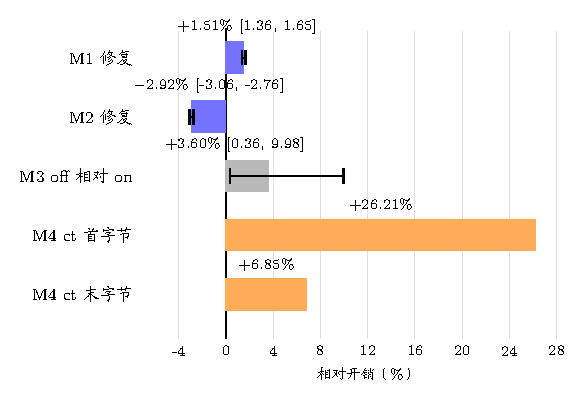
\includegraphics[width=0.92\textwidth]{assets/fig7.pdf}
\caption{防护前后成对相对开销}
\label{fig:overhead}
\par\smallskip
{\footnotesize 图注：M1 +1.51\%，M2 $-2.92\%$，M4 小内核 +26.21\%/+6.85\%。M3 的区间宽，只作描述；M4 是 32 B 比较调用，绝对差只有数纳秒，不能外推到完整解封装。}
\end{figure}

开销测量不是“前后各跑一次”。decaps 每臂 6 块 $\times$ 25,000 次，keygen 与 encaps 各 30,000 次，两臂按 ABAB 交错，相对开销用 bootstrap 10,000 次给区间。交错是为了让频率漂移、缓存状态与后台服务的影响同时落在两臂上；分块是为了让每块内部的顺序随机化。一次“修复前跑一遍、修复后跑一遍”的差值，无法区分防护开销与环境漂移。

M1 的 +1.51\% 可以拆成“多出的指令”与“多出的调用”。掩码选择把一条分支换成置位、取负、异或、与、再异或，指令数增加几条；16 位条件传送辅助函数在 -Os 下没有内联，多一次调用与返回。两部分加起来是 862.6 ns，占 57,010.7 ns 的 1.51\%。这个拆法只作解释，不作为精确归因；指令级开销要看反汇编与微基准。% A-25

M1 的 +1.51\% 是四次测量中最稳定的一个：区间窄，方向单一，与掩码选择多出的几条指令相符。M2 的修复反而更快，M3 的区间很宽，M4 的相对值很大但绝对差很小；三个对象的解释分别落在下面三段。

M2 的负开销来自编译器。除法被乘法与移位替代后，指令数减少，流水线停顿也减少；修复版反而比未修版快 2.92\%。这不等于“修复更安全”，只说明“更安全”与“更快”可以同向，也可以反向。把负开销写成“优化”会偏离主题：本作品测的是防护开销，不是性能优化。

M3 的 +3.60\% 区间 [0.36, 9.98] 很宽，是因为 off 臂的方差大、样本块少；这个区间只作描述，不用它推断总体开销。M3 是人工夹具，on/off 两臂只差一张查表；查表的开销在完整解封装里占比很小，测量噪声容易淹没它。把 3.60\% 写成“查表的开销”会高估精度。

M4 的 +26.21\% 与 +6.85\% 是相对值，绝对差只有 4 ns 量级。首字节与末字节的差异不同，是因为比较提前返回的位置不同：vulnerable 臂在第一个字节不同时最快返回，在最后一个字节不同时最慢；ct 臂始终遍历全部字节。两个百分比不能平均，也不能与完整解封装的百分比比较。

把相对开销换算成绝对时间：M1 每解封装多 862.6 ns，M2 少 1,690.5 ns；M3 的 +3.60\% 按 29,455.7 ns 的参考均值换算约 1.06 $\mu$s，但区间跨到 9.98\%，绝对量的不确定性也很大；M4 的 +26.21\% 只在小内核的比较调用上成立。绝对量与相对量一起看，才能判断这个开销在实际使用中的位置。% A-25 % B-02

M1 的 +1.51% 与 M2 的 −2.92% 方向相反，说明“防护一定变慢”不成立。掩码选择多出指令，除法替代减少指令；两个修复对指令数的影响不同，开销的方向也不同。把这两个数放在同一张图上，是为了让读者看到方向，而不是为了比较大小；不同对象的百分比不能直接排序。

M4 的 +26.21% 与 +6.85% 只用于说明“小内核的相对开销可以很大”。32 B 比较的基线远小于完整解封装，多几条指令就会带来 26% 的相对变化；换成 57 $\mu$s 的完整解封装，同样的指令数只占 0.0x%。相对开销必须绑定基线，脱离基线比较百分比没有意义。

开销的置信区间来自 bootstrap，不来自正态假设。M1 的区间 [1.36, 1.65] 窄，说明 6 块 $\times$ 25,000 次的成对测量稳定；M3 的区间 [0.36, 9.98] 宽，说明 off 臂的方差大、块数少。区间宽时只作描述，不用它推断总体；区间窄时也不把点估计当成精确值，只说明这次测量的相对开销落在那个范围。

表~\ref{tab:runtime} 同时给均值与分位数，是为了让读者看到分布的形状。均值对长尾敏感，分位数对长尾稳健；两者相差不大时，均值可以作为摘要；相差大时，分位数更能代表典型调用。这批数据的均值与中位数相差不到 100 ns，说明分布没有被长尾拉偏；如果只给均值，读者无法判断这一点。% A-25

性能开销不是本作品的目标，防护效果才是。开销测量的作用是回答“防护的代价有多大”，不是“哪个实现更快”；把 M2 的 $-2.92\%$ 写成“性能优化”会偏离主题。报告给开销区间，是为了让读者判断这个代价是否可以接受，而不是为了给实现排名。

五个对象的行不是同一把尺子。M1 与 M2 是完整解封装，可以互相比均值；M5 也是完整解封装，但实现不同，均值的差异主要来自参考路径，不来自防护；M3 与 M4 是小内核，只用于相对开销，不进入这张表。表~\ref{tab:runtime} 只列能放在同一窗口里比较的对象，跨对象的均值差不在结论里。

周期列只用于跨机器粗略对齐。周期按名义 4.30 GHz 换算，而实测频率中位数是 4,309,722.5 kHz，偏差 +0.005\%；用名义频率换算会带来同量级的系统误差。周期列不写进结论，也不与别的机器比较指令数；它只是让读者对“57 µs 在 4.30 GHz 下大约是多少个周期”有个量级概念。% A-31 % B-02

keygen 与 encaps 也做了测量，各 30,000 次，但表~\ref{tab:runtime} 只列 decaps。decaps 是防护的主要对象：M1 的分支、M2 的除法、M3 的查表、M4 的比较都在解封装路径上；keygen 与 encaps 的防护开销不是本轮重点。把 decaps 的开销写成“整个 KEM 的开销”会夸大适用范围。

开销测量与功能测试使用同一份产物；换构建要重测，这条约束与产物绑定一致。成对分块与 ABAB 交错解决的是“环境漂移”与“顺序效应”。如果先跑未修臂再跑已修臂，频率漂移、缓存升温与后台服务变化都会落在已修臂上；ABAB 让两臂在时间上交错，漂移同时落在两臂上。bootstrap 10,000 次给区间，不假设正态；区间窄说明相对开销稳定，不说明绝对耗时稳定。

表~\ref{tab:runtime} 的均值与图~\ref{fig:overhead} 的相对开销要一起读。均值给绝对量级，相对开销给可比的比例；只看均值，M1 与 M2 的差异只有 862.6 ns，容易被当成噪声；只看比例，+1.51\% 又缺少绝对量级。两者并排，读者才能判断“这个开销在 57 $\mu$s 里占多少”。% A-25 % B-02

表~\ref{tab:runtime} 与图~\ref{fig:overhead} 证明防护在本机带来的实测开销，以及成对设计能把环境漂移压到区间里；它们不证明开销低就一定安全，也不证明开销高就一定泄漏。M2 修复更快，不能写成“更安全”；M4 的百分比不能与完整解封装的百分比直接比较。

\subsection{编译选项与测量条件}
% A-26 优化级别 12 格
% A-29 锁频对照
% A-30 计时精度
% A-32 WSL2 复现
% B-11 优化矩阵

同一份源码在不同优化级别与测量条件下会呈现不同的产物形态与可检出性；结论必须绑定编译条件。图~\ref{fig:opt} 给出 12 格的合并均值差与 95\% 区间：M1 两版与 M5 各四个优化级别。% A-26 % B-11

\begin{figure}[htbp]
\centering
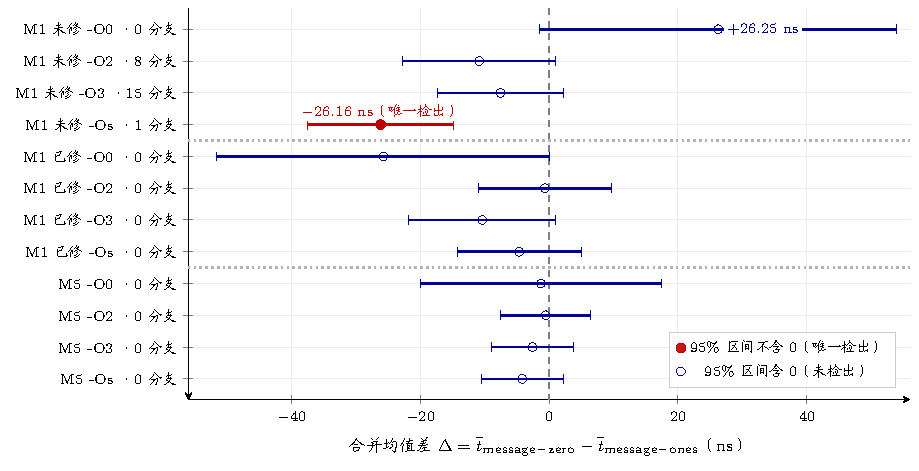
\includegraphics[width=0.98\textwidth]{assets/fig8.pdf}
\caption{优化级别 12 格合并均值差与 95\% 区间}
\label{fig:opt}
\par\smallskip
{\footnotesize 图注：只有 M1 未修 -Os 格区间不含 0；-O2/-O3 分支更多但计时未检出。区间为三个种子的逆方差合并；同一格三个种子使用同一份二进制。}
\end{figure}

12 格来自 3 个臂 $\times$ 4 个级别。3 个臂是 M1 未修、M1 已修与 M5；4 个级别是 -O0、-O2、-O3、-Os。每个格做产物判定（反汇编、除法计数、Memcheck）与锁频计时（每格 3 个种子），两列证据分开登记。

把产物判定与计时判定分开，是为了避免“分支存在但计时没测到”被读成“分支不存在”；-O2 与 -O3 正是这种情况。每格三个种子的二进制摘要逐字相同，判定用的产物与计时用的产物对齐；这一条是 12 格可比的前提；换优化级别或编译器都要重新登记产物，这条约束不随环境改变。

12 格是族外探索，不进任何 Holm 家族。它的作用是看“产物形态与可检出性是否随编译条件变化”，不是给每个优化级别下安全结论；每格 3 个种子，样本量不足以做家族检验，也不足以估计总体。结论止于“该级别下没有观察到可区分差异”。

M1 未修的 -Os 格合并 $-26.16$ ns，区间 [$-37.51$, $-14.81$]，是 12 格中唯一不含 0 的区间；同一版本的 -O2 与 -O3 分别合并 $-10.86$ 与 $-7.55$ ns，区间都含 0；-O0 没有秘密相关分支，源码的算术掩码被原样保留。产物侧，-O2 与 -O3 的秘密相关分支位置数为 8 与 15，比 -Os 的 1 个更多；分支更多，计时反而未检出。修复版四个级别都是 0 个秘密相关分支，M5 四个级别都是 0，12 格都没有整数除法指令。% A-26

其余 11 格的区间同样列出。M1 未修 -O0 合并 +26.25 ns，区间 [$-1.42$, 53.92]；-O2 $-10.86$ [$-22.75$, 1.02]；-O3 $-7.55$ [$-17.35$, 2.26]。M1 已修 -O0 合并 $-25.75$ [$-51.59$, 0.09]，上界紧贴 0；-O2 $-0.69$ [$-11.02$, 9.63]；-O3 $-10.38$ [$-21.77$, 1.00]；-Os $-4.64$ [$-14.29$, 5.02]。

M5 四格都在 $-5$ ns 以内，区间都含 0。只有 -Os 未修格的距离离 0 足够远。

“分支更多反而未检出”有两层解释。产物层：-O2/-O3 的每比特测试是“内存操作数加条件跳转”，形态与 -Os 的寄存器位测试不同；分支数量多，不等于单条分支的代价大。计时层：分支的代价被流水线、分支预测与乱序执行吸收，端到端均值差可能小于 MDE；-O2/-O3 的区间都含 0，说明这个预算下没有分辨出来。两层解释都指向同一个结论：不能从“分支数量”推断“可检出性”。

锁频与不锁频的对照给出另一个反直觉结果。三个对象的 CV 比为 0.964、1.006、1.089，SD 比为 0.741、0.757、0.956；不锁频的标准差反而更低。M1 未修在两种条件下都是 3/3 检出，M5 都是 0/3；判定一致，稳定性指标的方向却不一致。% A-29

CV 比的方向不一致，说明“锁频降噪”这个直觉在这台机器上不成立：M1 未修 0.964、M1 已修 1.006 小于或等于 1，M5 1.089 大于 1；如果锁频一定降噪，三个比值应该都大于 1。SD 比都小于 1，是因为不锁频时频率更高、单次调用更短，绝对标准差随均值一起缩小；换成 CV 后，两者的相对离散度接近。锁频真正提供的是可核对的工作点：每次运行记录 20 次探针、退出核对恢复，审计者能确认“这次采集在什么频率下完成”。

-O0 格没有秘密相关分支，是“该级别下这个机制没有出现”，不是“这份源码安全”。源码的算术掩码被原样保留，编译器没有把它还原成条件跳转；换一个编译器或换一个 -march，-O0 也可能出现分支。把 -O0 的 0/0 写成“最安全的级别”会越过产物边界；本作品只写“该级别下没有观察到该机制”。

修复版四个级别都是 0 个秘密相关分支，说明官方修复在不同优化级别上都生效；它不说明修复版在计时层也不可区分。M1 已修的四个级别合并值分别为 $-25.75$、$-0.69$、$-10.38$、$-4.64$ ns，区间都含 0；这是产物层与计时层分开登记的结果。产物层 0 个分支、计时层区间含 0，两者同向，但不能互相替代。

三台 WSL2 虚拟化环境的复现把“机制”和“可检出性”分开。确定性证据与主平台一致：M1 未修 -Os 1 个、-O2 8 个、-O3 15 个、-O0 0 个 Memcheck 上下文，修复版与 M5 全为 0，反汇编形态逐项相同。时间证据不同：三台机器上 M1 未修 -Os 的合并区间都含 0，M4 vulnerable 的合并区间都不含 0（$-7.13$、$-11.97$、$-22.37$ ns）。机制存在与否可以跨环境复现，数十纳秒效应的可检出性依赖测量环境；WSL2 数据不进任何 Holm 家族，也不与裸金属数据合并。% A-32

WSL2 的三台机器不是三台测量机。它们是虚拟化环境，不锁频，时间数据的标准误在数百纳秒；三台机器的一致之处是确定性证据（反汇编、Memcheck），不是时间证据。M4 vulnerable 在三台机器上都给出不含 0 的区间，说明管线在效应足够大时仍能检出；M1 未修 -Os 的区间都含 0，说明 32 ns 效应在虚拟化噪声下不可检出。

WSL2 的结果还说明“效应足够大时管线仍能检出”。M4 的 4 ns 效应在虚拟化噪声下仍能给出不含 0 的区间，是因为比较调用的方差小、信噪比高；M1 的 32 ns 效应在 WSL2 上反而测不到，是因为完整解封装的方差大、虚拟化噪声高。可检出性不是只由效应绝对值决定，还由噪声与样本量决定；同一台机器上，M4 的 MDE 比 M1 小两个数量级，原因就在这里。

计时精度决定了什么样的效应可以被讨论。读钟开销约 17.4 ns，最小步进 10 ns；时间戳计数器的速率为 4,291,962 kHz，单次读数的分辨率下界为 42--43 个计数、约 9.8--10.0 ns；1 ms 短区间的频率极差为 348 kHz，相对标准差 $5.4\times10^{-6}$。逐调用物理恒频不可主张：锁频协议固定的是工作点，不是每一次调用的频率。% A-30

时间戳计数器的读数不是物理时间的直接测量。TSC 速率 4,291,962 kHz 是按名义频率校准的；单次读数 42--43 个计数对应 9.8--10.0 ns，是分辨率下界，不是精度。1 ms 短区间的频率极差 348 kHz、相对标准差 $5.4\times10^{-6}$，说明短窗内频率稳定；长期稳定性没有认证，逐调用物理恒频不可主张。

锁频/不锁频对照每组只有 3 次运行，只作描述。3 次运行不足以估计总体方差，也不足以推断其他处理器或调速策略；CV 比 0.964--1.089 只能说明“这台机器上方向不一致”，不能说明“锁频在所有机器上都不降噪”。把这条对照写成普遍结论，会超出样本边界。

图~\ref{fig:opt} 与这组对照证明产物与测量条件会改变可检出性；它们不证明某个优化级别绝对安全，也不证明其他编译器、其他 CPU 会给出同样的结果。本机未配置 isolcpus，SMT 开启，后台约 39 个服务在运行；这些条件与 10 ns 量化一起，构成时间证据的环境边界。

\subsection{架构与网络边界}
% A-27 aarch64 12 格
% A-28 同机网络五档
% A-30 计时精度
% B-03 检测预算
% B-12 网络档位

M1 的泄漏机制是 x86\_64 特定的编译器产物；同机网络各档在本预算下未检出，不能外推真实远程。图~\ref{fig:boundary} 把架构对照与网络检测预算放在一起：左侧是同一份源码在两个架构上的产物形态，右侧是五档网络分辨同一量级效应所需的样本数。% A-27 % A-28

aarch64 的实验条件是“真指令集、原生二进制”。它在 Apple Silicon 的容器内运行，运行时报告的机器类型是 aarch64，不是 QEMU 翻译，也不是交叉编译后在 x86\_64 上跑；同一份 liboqs 0.10.0 源码、同一个 clang 18、同一组优化级别，只换架构。这个条件让“产物形态不同”可以归因到架构，而不是源码或编译器版本。

容器环境的限制要写明：没有锁频，没有裸金属，CPU 与其他容器共享；这些条件不影响确定性证据（反汇编、Memcheck），但影响时间证据。aarch64 的 12 格只做产物判定与 Memcheck，不做锁频计时；把它的时间数据与 x86\_64 合并会引入不可控的环境差异。

\begin{figure}[htbp]
\centering
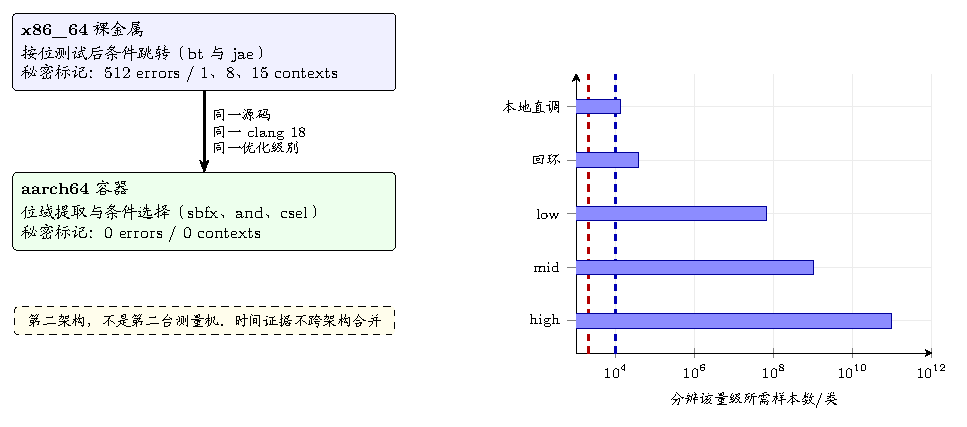
\includegraphics[width=0.99\textwidth]{assets/fig9.pdf}
\caption{架构与网络边界}
\label{fig:boundary}
\par\smallskip
{\footnotesize 图注：x86\_64 的 bt/jae 在 aarch64 上变为 sbfx/csel；网络各档在本预算下未检出。右侧虚线为本轮实际样本数（网络每类 2,000，本地直调每类 10,000）。}
\end{figure}

aarch64 的 12 格全部是 0 errors / 0 contexts；x86\_64 同格的 M1 未修是 512 errors / 8、15、1 个上下文。反汇编上，x86\_64 是按位测试后条件跳转（bt 与 jae），aarch64 是位域提取、与掩码、条件选择（sbfx、and、csel），消息位的选择全部走无分支算术。同一份源码、同一个 clang 18、同一个优化级别，产物性质不同；M1 的机制不是“ML-KEM 参考实现在别的架构上也泄漏”，而是 x86\_64 编译器在特定选项下的产物。

x86\_64 的 512 errors / 8、15、1 个上下文，对应 -O2、-O3、-Os 三个级别；aarch64 同格都是 0/0。-O0 在两个架构上都是 0，因为源码的算术掩码被原样保留。三个不一致的格子全部落在“x86\_64 加 M1 未修”，这个分布说明差异绑定的是架构与产物的组合，不是探针或输入。

12 格里 9 格一致、3 格不一致，不一致的全部集中在 x86\_64 的 M1 未修臂。这个分布本身就是证据：如果差异来自探针或环境，应该在各臂上随机出现；差异只在“x86\_64 加 M1 未修”这一组出现，说明它绑定的是产物形态，不是测量环境。aarch64 上消息位选择走无分支算术，Memcheck 没有秘密相关分支可报，0/0 是产物性质的结果。

aarch64 上 0/0 的原因可以直接从反汇编读出来：消息位的选择走位域提取、与掩码、条件选择，三个步骤都不产生依赖秘密的跳转；Memcheck 没有秘密条件跳转可报，也没有秘密下标可报。0/0 不是“工具没跑”或“输入没覆盖”，而是“产物里没有这个机制”；同一份探针在 x86\_64 上报 512 errors，说明探针本身有效。

aarch64 跑在容器内，未锁频，不是裸金属；它只构成第二架构，不是第二台测量机。跨架构的时间证据不合并，也不要求同号；两个架构的探针实现不完全相同，M5 的跨架构结论只能由“两架构都是 0”弱支撑，不能写成强结论。把 aarch64 写成“第二台测量机”会夸大证据：它没有锁频，没有裸金属，时间数据不进入任何家族。

两个架构的探针实现不完全相同：x86\_64 的 M5 四格用另一个探针，aarch64 用同一份历史探针；M5 的跨架构结论只能由“两架构都是 0”弱支撑。两架构都是 0 只支持“未检出”；探针不同，不能升级为常数时间结论。

同机网络场景用裸金属、匿名网络命名空间、自有 veth 与内核 netem 构造两端 TCP，分五档：本地直调、回环、low、mid、high。本地直调档 M1 未修两次运行一次可分辨（+37.1 ns，区间 [20.4, 53.8]）、一次未检出（$-7.9$ ns，区间 [$-25.0$, 9.2]）；网络各档全部未检出。分辨同一量级效应所需的每类样本数为 13,098、38,417、64,636,555、1,003,153,317、97,586,175,893；网络各档实际每类 2,000，比所需少 1.3--7.7 个数量级。% B-03 % B-12

网络拓扑是同机两端：服务端在匿名 netns 内，绑到锁频 CPU2；客户端在宿主 netns，绑到 CPU0/1/3，不占 CPU2/CPU6。veth 两端用一对私有 /30 地址；netem 挂在 veth 两端，单向延迟与抖动分别是 100 $\mu$s/20 $\mu$s、1 ms/200 $\mu$s、10 ms/2 ms。这个拓扑能加入协议栈、排队与链路抖动，不能加入真实广域网的拥塞与路由变化。

网络五档的设计是为了分离“协议栈”“排队”与“链路抖动”三项开销。本地直调不走 socket，回环走 veth 与 TCP 但不加 netem，low/mid/high 逐级加入延迟与抖动；五档的检测预算逐级上升，说明每加入一层开销，分辨同一效应所需的样本数就增加。这个阶梯是定性的，不是对真实网络的拟合。

本地直调档的两次运行给出了两种结果：一次 +37.1 ns、区间 [20.4, 53.8]，一次 $-7.9$ ns、区间 [$-25.0$, 9.2]。两次的噪声水平接近，差别来自效应本身的运行间变动；把两次合并得到的参照效应区间含 0，只能当量级参照。这段结果说明：即使在同一台机器、同一锁频工作点，32 ns 级效应的可分辨性也不是每次都稳定；网络档每类只有 2,000，更不可能稳定分辨。

网络档的 netem 参数是单向 100 µs/20 µs、1 ms/200 µs、10 ms/2 ms，三档对应 low、mid、high。回环档不走 netem，只有 veth 与 TCP 的开销；本地直调档不走 socket，直接调用解封装。五档的设计是为了让“协议栈与排队”逐级加入，而不是一步跳到真实远程。即使最轻的回环档，所需样本数也比实际多 1.3 个数量级；加上 netem 后，所需样本数上升到 $10^7$--$10^{11}$，实际每类 2,000 远远不够。

检测预算按 $n=2(1.96\,\mathrm{SD}/|\Delta|)^2$ 计算，与 MDE 同口径；本地直调 13,098、回环 38,417、low 64,636,555、mid 1,003,153,317、high 97,586,175,893。网络各档实际每类 2,000，回环差 1.3 个数量级、low 差 4.5 个、mid 差 5.7 个、high 差 7.7 个。预算数字不是“需要这么多才能攻击”，是“需要这么多才能分辨这个量级的差异”；两者不能混。

网络档每类 2,000 的样本量是预算与机时的折中。按本地直调的 13,098 所需样本，2,000 只有 0.15 倍；按 high 档的 97,586,175,893，2,000 差 7.7 个数量级。样本量不足时，未检出是预期结果，不是“网络没有泄漏”的证据；报告把预算与差距一起写出，是为了让读者自己判断这个阴性有多强。

netem 的三档不是“轻度、中度、重度网络”的通用定义，是本作品选的三组参数。low 档 100 $\mu$s/20 $\mu$s 接近同城链路，mid 档 1 ms/200 $\mu$s 接近跨城，high 档 10 ms/2 ms 接近跨洲；这些类比只用于读者建立量级感，不是真实测量。真实远程的排队、拥塞与路由变化不在这个拓扑里。

这是同机模拟，不是真实远程；网络各档的“未检出”只说明在本预算下没有看到可区分差异，不说明远程链路上不存在泄漏，也不说明远程攻击不可行。图~\ref{fig:boundary} 证明机制与可检出性有环境边界；它不证明远程攻击可行或不可行，也不证明某个架构绝对安全。在同机模拟里，网络各档的检测预算比实际样本高 1.3--7.7 个数量级；在真实远程里，链路抖动、拥塞与路由变化只会让预算更高，不会更低。这个方向性判断不依赖具体数字，但它是推断，不是实测；本作品不把它写成“远程不可测”。

\subsection{多工具交叉验证}
% A-16 RTLF
% A-24 工具矩阵
% B-04 RTLF 数据集
% B-05 工具矩阵分解

单工具会给出方向相反的读法；交叉矩阵的价值不是“工具多”，而是让每个工具的“回答什么、不回答什么”落在同一张表上。图~\ref{fig:tools} 是 9 工具 $\times$ 5 模块的矩阵：30 格有真实运行产物，15 格未运行。% A-24 % B-05

\begin{figure}[htbp]
\centering
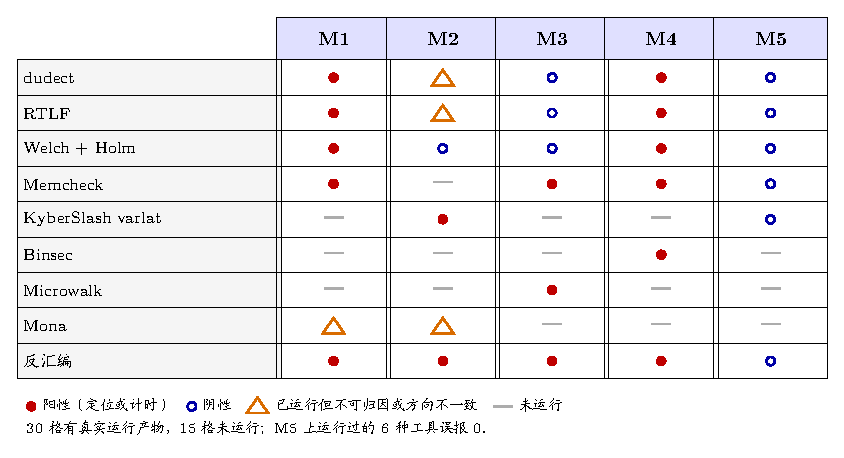
\includegraphics[width=0.96\textwidth]{assets/fig10.pdf}
\caption{多工具交叉矩阵}
\label{fig:tools}
\par\smallskip
{\footnotesize 图注：30 格有真实产物，15 格未运行；M5 上 6 工具误报 0。阳性指该工具在其判定层报告了机制或可区分性，阴性指未报告；未运行不等于阴性。}
\end{figure}

矩阵的 9 个工具分三类：族内统计（Welch+Holm）、族外统计（dudect、RTLF、Mona）、定位工具（反汇编、Memcheck、varlat、Microwalk、Binsec）。三类回答的问题不同，矩阵把它们放在同一组模块上，是为了看“同一对象在不同判据下会不会给出相反读法”。15 个未运行格都写了原因：M2 没有完整解封装的 Memcheck 探针，M1/M2 没有 Binsec 抽取内核，M3/M4/M5 没有接入 Microwalk，Mona 只接入 M1/M2。未运行格不填阴性。矩阵按 2026-10-16 冻结的产物登记；M5 上的有界验证结果在矩阵冻结后补充，列在 3.4，不计入这张矩阵的 30 格与 6 工具统计。矩阵的格数不随补充结果改变；未运行格也不因补充结果改填阴性。

三类工具的回答范围不同。族内统计回答“均值差是否可区分”，族外统计回答“分布是否不同”，定位工具回答“哪里依赖秘密”。同一格在族内统计是阴性、在族外统计是阳性，不是矛盾：它们比较的对象不同。矩阵把三类放在一起，是为了让读者看到“同一对象在不同判据下可以给出不同读法”，而不是让它们投票。

M1 是五路同向的例子：反汇编看到按位测试后条件跳转，Memcheck 看到 1 个秘密条件跳转，Welch+Holm 拒绝主类对，RTLF 在未修臂报告差异、在已修臂未报告，dudect 最大 $t$ 在未修臂为 26.41、40.64、14.92、在已修臂为 1.15、1.12、1.31。五类工具回答的问题不同，结论同向。

五路同向增加信心，但不等于“五倍证据”：它们共享同一份产物与同一组输入，不是五个独立实验。

M4 是人工夹具中唯一定位层与计时层都阳性、ct 臂全阴性的正对照。M5 上运行过的 6 种工具全部阴性，误报 0；这个数字只说明这 6 种工具在这个对象、这些输入上没有报假阳性，不能估计总体误报率。

M4 的正对照作用是把“定位阳性”与“计时阳性”同时钉在一个对象上。如果 M4 的 ct 臂也阳性，说明检测链路有假阳性；如果 vulnerable 臂阴性，说明链路测不到已知机制。两种失败都没有出现，M4 才能作为正对照。M5 的阴性对照作用相反：如果 6 种工具在 M5 上报阳性，说明工具有误报；6 种都报 0，说明本次没有误报。

误报 0 的分母是 6 个工具 $\times$ 1 个对象，不是 6 个工具 $\times$ 全部输入。M5 上每种工具只跑了一组输入或一个探针；换一组输入、换一个优化级别，误报率可能不同。把“6 工具误报 0”写成“工具不会误报”会越过样本边界；写成“本次未出现误报”才是准确的。

单工具误读在 M2 上最清楚。只看 RTLF，会把 M2 读成“两臂都可区分”：主类对 6/6 检出，未修与已修各 3 次；只看 dudect，会因阳性落在已修臂（36.27、30.94、61.91 对 4.68、3.05、3.66）而得出“修复引入泄漏”。两个读法都与端到端 Welch 检验的未检出冲突。\cite{dudect}

Mona 的不一致原样保留。M1 未修臂全部无分离、已修臂 2/6 次分离，与 Welch、RTLF、dudect 的方向都不一致；它的“置信”字段是批次成功百分比，不是 $p$ 值，不能参与 Holm，也不能用来推翻既有结论。把 Mona 的不一致写成“工具有问题”或“结论有问题”都越界；它只说明这个工具的判据与另外三类不同。

M2 的两个误读来自不同的判据。RTLF 比较分布与分位，主类对使消息位走系统性不同的路径，分布差异可能来自分支而不是除法；dudect 用在线 $t$ 检验，阳性落在已修臂，说明它测到的是修复引入的另一种差异，不是除法。两个工具都没有定位到除法热点；把它们与 Memcheck、varlat 的定位结论交叉，才能得到“定位阳性、计时未检出”的完整读法。

15 个未运行格分布在 5 个工具上：Memcheck 缺 M2 的完整解封装探针，varlat 缺 M1/M3/M4，Binsec 缺 M1/M2/M3/M5，Microwalk 缺 M1/M2/M4/M5，Mona 缺 M3/M4/M5。每一格都写了原因；补上它们需要额外的探针、抽取内核或工具接入。未运行格不是阴性，也不是“无关紧要”；它们只是本轮没有数据。

图~\ref{fig:tools} 证明多工具交叉能消除单工具误读，并把“未运行”与“阴性”分开；它不证明所有工具都同意，也不证明没有假阴性。15 格未运行不等于阴性，未运行格只写原因，不填结论。补上这些格需要额外的工具安装与模型构建，本作品没有做。

交叉矩阵不产生新的统计判定。它把已有工具的结论放在同一张表上，让读者看到“同一对象在不同判据下可以给出不同读法”；它不做投票，也不把多数工具的意见当成结论。主结论仍由预注册 Holm 家族给出，矩阵只负责解释与边界。

\subsection{可复现性}
% A-37 干净 clone 与匿名包
% B-09 测试总数

可复现不是“代码在仓库”，而是“干净 clone 能跑、包内能复算、每个数字能回到原始行”。一键入口分 quick 与 full 两档：quick 不写 sysfs、不绑核，用固定输入跑功能与统计复算；full 需要锁频控制器与裸金属硬件，按冻结计划重采时间数据。

quick 档的设计目标是“在任何一台能编译的机器上跑通软件流程”。它不写 sysfs，不需要 root，不绑核；它跑功能测试、统计重算与报告生成，不产生新的时间结论。full 档才需要锁频控制器、裸金属与固定的 CPU；它按冻结计划重采，产出原始长表与运行台账。两档分开，是为了让“软件流程可复现”与“时间结论可复现”不混为一谈：前者任何机器都能做，后者需要硬件。

quick 档的输入是固定的，输出是功能测试结果与统计重算结果；它不产生新的时间数据，因此不需要锁频。full 档的输入是冻结计划，输出是原始长表与运行台账；它需要锁频控制器、绑核与恢复核对。两档的入口是同一个脚本，参数不同；把两档分开，是为了让读者知道“跑通”与“复现时间结论”是两件事。

干净 clone 的四个测试集合计 263 项通过、0 失败：platform 88、ordinary 57、sanitize 57、historical-fixed 61。匿名包解出后 CTest 5/5。随包提供 42 份原始长表、逐次运行台账、冻结计划、产物摘要与统计脚本；每个正文数字可以按附录 B 的运行编号回到原始行，统计判定可以按附录 C 的公式与脚本复算。% A-37 % B-09

42 份原始长表是逐次运行的原始值，不是汇总表；每份长表带运行编号、模块、臂、种子、CPU 与产物摘要。逐次运行台账记录每次控制器运行的进入、采中、退出三段；冻结计划记录主类对、样本量、停止条件与 Holm 家族；统计脚本按附录 C 的公式重算。四类材料合起来，第三方可以从原始值走到正文数字。

263 项测试是软件流程验证，不是计时复现。platform 88 项覆盖平台自身的构建与接口，ordinary 57 项覆盖普通构建，sanitize 57 项覆盖 ASan/UBSan 构建，historical-fixed 61 项覆盖历史修复版；四类合起来说明代码在各构建配置下能跑、功能测试能过，不说明时间结论能在别的机器上复现。263 项证明的是流程，不是时间。

复现边界要写清楚：完整锁频采集需要硬件，包内不能代替；外部 RTLF、Mona、dudect、Binsec 不在包内重跑，只保留输出摘要与调用参数；包内复算只重算已有数据，不产生新实验。这组结果证明软件流程与统计判定可复算，不证明任何机器都能复现时间结论；时间结论依赖本机、本编译产物与锁频工作点。

匿名包解出后 CTest 5/5，是包内复算的入口。它验证包内构建、功能测试与统计脚本能在干净环境里跑通；它不重跑外部工具，也不重采时间数据。5/5 说明包内流程可复算，不覆盖外部工具与时间数据。
